% This is a UHH LaTeX thesis template (English) that is built on the template 
% of the UHH informatics department and the template of the Reed 
% College LaTeX thesis (from the thesisdown R package).

% -------------------------------
% --- PREAMBLE ---
% -------------------------------
\documentclass[a4paper,12pt]{article}


% Coding, Language, Patches {{{
\usepackage[T1]{fontenc}    % for coding output; allows for umlaut, accents und
                            % correct hyphenation
\usepackage[utf8]{inputenc} % allows for direct input of special characters; 
\usepackage[ngerman, english]{babel} 
\usepackage{microtype}      % Optimale margin and scale setting
\usepackage[autostyle]{csquotes}  % Correct quotation marks in bibliograpy
\usepackage{scrhack}        % Avoids warnings with older packages
\usepackage[newcommands]{ragged2e}  % Improves \ragged...commands
\PassOptionsToPackage{hyphens}{url}   % for URL line breaks in footmarks and bibliography
% }}}

% Fonts {{{
\usepackage{mathptmx}       % Times; modifies the default serif and math fonts
\usepackage[scaled=.92]{helvet}% modifies the sans serif font
\usepackage{courier}        % modifies the monospace font
\usepackage{sectsty}        % the alternative with {titlesec} did not work
% make headers same style as in scrreprt document class:
\sectionfont{\sffamily\bfseries}
\subsectionfont{\sffamily\bfseries}
\linespread{1.25}               % make line hight equivalent to 1.5 in MS Word
% }}}

% Document and text settings {{{
\usepackage[
    a4paper,
    margin=2.5cm,
    marginparwidth=2.0cm,
    footskip=1.0cm
    ]{geometry}           
\clubpenalty=10000          % avoids so-called 'clubs': single lines at beginning of paragraph
\widowpenalty=10000         % avoids so-called 'widos': single lines at end of paragraph
\displaywidowpenalty=10000
\usepackage{ifdraft}        % enables \ifoptionfinal{true}{false}
\pagestyle{plain}           % no headlines
\setlength{\emergencystretch}{3em} % prevent overfull lines
% }}}

% Table packages {{{
\usepackage{booktabs}			% for publication quality tables in LaTeX
%\usepackage{tabu}           % Einfügen von Tabellen.
\usepackage{tabularx} 			% defines an environment tabularx, an extension of tabular
\usepackage{longtable}    % handles multipage tables
\usepackage{multirow}       % % creates tabular cells spanning multiple rows
\usepackage{multicol}       % % creates tabular cells spanning multiple columns
 \usepackage{array}				% extends the array and tabular environments
% }}}

% % Other packages {{{
\usepackage{amsmath,amssymb,amsthm}    % Typical maths resource packages
\usepackage{calc}				% for simple arithmetic in LaTeX commands
\usepackage{textcomp}                           % For single quotes
\usepackage[bf]{caption}
\usepackage[bottom, flushmargin]{footmisc}      % For footnotes
\usepackage{footnotebackref}
\usepackage{tikz}				% tool to create graphic elements in LaTeX
% }}}

% URLs {{{
\usepackage[hyphens]{url}
\urlstyle{same} % disable monospaced font for URLs
% }}}

% define topline
% \usepackage[automark]{scrlayer-scrpage}
% \pagestyle{scrheadings}
% \automark{section}
% \clearscrheadings
% \ohead{\headmark}

% Define citation style {{{
\usepackage{natbib}       % literature reference style
  \bibliographystyle{}
  \bibliography{bib/references.bib}
% }}}

% ToC {{{
\setcounter{secnumdepth}{5}
\setcounter{tocdepth}{5}
% }}}

  \usepackage[parfill]{parskip}


% Graphics {{{
\usepackage{graphicx}            % Packages to allow inclusion of graphics
\makeatletter
\def\maxwidth{\ifdim\Gin@nat@width>\linewidth\linewidth\else\Gin@nat@width\fi}
\def\maxheight{\ifdim\Gin@nat@height>\textheight\textheight\else\Gin@nat@height\fi}
\makeatother

% define position of graphics
\usepackage{float}
\floatplacement{figure}{H}
\floatplacement{table}{H}
% to change the default alignment of a image
\usepackage[export]{adjustbox}
% }}}


% Colors {{{
\usepackage{xcolor}			% extends LATEX's color facilities
\usepackage{colortbl}			% to add colour to LaTeX tables

% define colors for hyperlinks:
\definecolor{linkcol}{HTML}{014979} %darkblue
\definecolor{filecol}{HTML}{b70000} %darkred
\definecolor{urlcol}{HTML}{b70000} %darkred
\definecolor{citecol}{HTML}{4c4c4c} %darkgray


% Hypersetup
\hypersetup{
colorlinks=true,
linkcolor=linkcol,
filecolor=filecol,
urlcolor=urlcol,
citecolor=citecol,
linktocpage=true,
pdfpagemode=UseOutlines,
}

% }}}

% Cross-referencing {{{
% Use ref for internal links
\usepackage{hyperref}     % to handle cross-referencing commands in LaTeX
\renewcommand{\hyperref}[2][???]{\autoref{#1}}
\def\chapterautorefname{Chapter}
\def\sectionautorefname{Section}
\def\subsectionautorefname{Subsection}
% }}}


% Define tightlist to work with newer versions of pandoc
\providecommand{\tightlist}{%
  \setlength{\itemsep}{0pt}\setlength{\parskip}{0pt}}
  
% Save thesis parameters for later
\newcommand{\thesistype}{Bachelor's / Master's Thesis}
\newcommand{\thesisauthor}{Mandy Mustermann}
\newcommand{\thesisdate}{}




% Syntax highlighting 
  \usepackage{color}
  \usepackage{fancyvrb}
  \newcommand{\VerbBar}{|}
  \newcommand{\VERB}{\Verb[commandchars=\\\{\}]}
  \DefineVerbatimEnvironment{Highlighting}{Verbatim}{commandchars=\\\{\}}
  % Add ',fontsize=\small' for more characters per line
  \usepackage{framed}
  \definecolor{shadecolor}{RGB}{248,248,248}
  \newenvironment{Shaded}{\begin{snugshade}}{\end{snugshade}}
  \newcommand{\AlertTok}[1]{\textcolor[rgb]{0.94,0.16,0.16}{#1}}
  \newcommand{\AnnotationTok}[1]{\textcolor[rgb]{0.56,0.35,0.01}{\textbf{\textit{#1}}}}
  \newcommand{\AttributeTok}[1]{\textcolor[rgb]{0.77,0.63,0.00}{#1}}
  \newcommand{\BaseNTok}[1]{\textcolor[rgb]{0.00,0.00,0.81}{#1}}
  \newcommand{\BuiltInTok}[1]{#1}
  \newcommand{\CharTok}[1]{\textcolor[rgb]{0.31,0.60,0.02}{#1}}
  \newcommand{\CommentTok}[1]{\textcolor[rgb]{0.56,0.35,0.01}{\textit{#1}}}
  \newcommand{\CommentVarTok}[1]{\textcolor[rgb]{0.56,0.35,0.01}{\textbf{\textit{#1}}}}
  \newcommand{\ConstantTok}[1]{\textcolor[rgb]{0.00,0.00,0.00}{#1}}
  \newcommand{\ControlFlowTok}[1]{\textcolor[rgb]{0.13,0.29,0.53}{\textbf{#1}}}
  \newcommand{\DataTypeTok}[1]{\textcolor[rgb]{0.13,0.29,0.53}{#1}}
  \newcommand{\DecValTok}[1]{\textcolor[rgb]{0.00,0.00,0.81}{#1}}
  \newcommand{\DocumentationTok}[1]{\textcolor[rgb]{0.56,0.35,0.01}{\textbf{\textit{#1}}}}
  \newcommand{\ErrorTok}[1]{\textcolor[rgb]{0.64,0.00,0.00}{\textbf{#1}}}
  \newcommand{\ExtensionTok}[1]{#1}
  \newcommand{\FloatTok}[1]{\textcolor[rgb]{0.00,0.00,0.81}{#1}}
  \newcommand{\FunctionTok}[1]{\textcolor[rgb]{0.00,0.00,0.00}{#1}}
  \newcommand{\ImportTok}[1]{#1}
  \newcommand{\InformationTok}[1]{\textcolor[rgb]{0.56,0.35,0.01}{\textbf{\textit{#1}}}}
  \newcommand{\KeywordTok}[1]{\textcolor[rgb]{0.13,0.29,0.53}{\textbf{#1}}}
  \newcommand{\NormalTok}[1]{#1}
  \newcommand{\OperatorTok}[1]{\textcolor[rgb]{0.81,0.36,0.00}{\textbf{#1}}}
  \newcommand{\OtherTok}[1]{\textcolor[rgb]{0.56,0.35,0.01}{#1}}
  \newcommand{\PreprocessorTok}[1]{\textcolor[rgb]{0.56,0.35,0.01}{\textit{#1}}}
  \newcommand{\RegionMarkerTok}[1]{#1}
  \newcommand{\SpecialCharTok}[1]{\textcolor[rgb]{0.00,0.00,0.00}{#1}}
  \newcommand{\SpecialStringTok}[1]{\textcolor[rgb]{0.31,0.60,0.02}{#1}}
  \newcommand{\StringTok}[1]{\textcolor[rgb]{0.31,0.60,0.02}{#1}}
  \newcommand{\VariableTok}[1]{\textcolor[rgb]{0.00,0.00,0.00}{#1}}
  \newcommand{\VerbatimStringTok}[1]{\textcolor[rgb]{0.31,0.60,0.02}{#1}}
  \newcommand{\WarningTok}[1]{\textcolor[rgb]{0.56,0.35,0.01}{\textbf{\textit{#1}}}}

% Additional LaTeX parameters added in the YAML header of index.Rmd



\begin{document}

% -------------------------------
% --- frontmatter: Title page ---
% -------------------------------
\thispagestyle{empty}
\begin{titlepage}


\includegraphics[width=6.8cm]{images/uhh_logo.png}
\hspace{2cm}

\includegraphics[width=7cm]{images/min_logo.png}
\begin{center}\Large
  \vfill
	Bachelor's / Master's Thesis
	\vfill
	\makeatletter
	{\LARGE\textsf{\textbf{Thesis title}}\par}
	\makeatother
	\vfill
  submitted by \\\vspace{0.5cm}
  \par\bigskip
	\makeatletter
  \textbf{Mandy Mustermann} \\
  \makeatother
  born on 31. January 1970 \\
  Matriculation number: 1234567 \\
  Degree program: Biology \\
  \vfill
	\makeatletter
	submitted on 1. April 2000
	\makeatother
	\vfill
  1. Advisor: Prof.~Dr. \\
  2. Advisor: Prof.~Dr. \\

\end{center}
\end{titlepage}

% -----------------------------
% --- frontmatter: Abstract ---
% -----------------------------
\newpage
\hypertarget{abstract}{%
\section*{Abstract}\label{abstract}}
\addcontentsline{toc}{section}{Abstract}

The abstract comes always first and should raise the readers interest in reading further.

The abstract summarizes, usually in one or two paragraph (here max. 1 page), the major aspects of the entire thesis in a prescribed sequence. This should include:
\begin{itemize}
\tightlist
\item
  the overall purpose of the study and the research problem(s) you investigated
\item
  the basic design of the study
\item
  the major findings or trends found as a result of your analysis
\item
  a brief summary of your interpretations and conclusions.
\end{itemize}
\pagestyle{plain}
\pagenumbering{roman}   % define page number in roman style
\setcounter{page}{1}    % start page numbering

% ------------------------------------
% --- frontmatter: Zusammenfassung ---
% ------------------------------------
\newpage
\hypertarget{zusammenfassung}{%
\section*{Zusammenfassung}\label{zusammenfassung}}
\addcontentsline{toc}{section}{Zusammenfassung}

The thesis should always provide a German summary after the abstract, independent of the language of the main sections. Its content should not deviate from the abstract.

% -----------------------------
% --- frontmatter: Contents ---
% -----------------------------
\newpage
\renewcommand{\contentsname}{Table of Content}
\tableofcontents
\clearpage

% ----------------------------------------------------------
% --- frontmatter: List of Abbreviations (not mandatory) ---
% ----------------------------------------------------------
\newpage
\hypertarget{list-of-abbreviations}{%
\section*{List of Abbreviations}\label{list-of-abbreviations}}
\addcontentsline{toc}{section}{List of Abbreviations}

You can provide a table of abbreviations in R Markdown syntax or \LaTeX syntax. But if you do the former, R will count this table and, consequently, the next actual table will start with the counter 2:

\vspace{1cm}
\begin{tabular}{*2{l}}
    ATP  &  Adenosine Triphosphate   \\ 
    CoA  &  Coenzyme A  \\
    DNA  &  Deoxyribonucleic Acid \\         
    mtDNA  &  Mitochondrial DNA \\
\end{tabular}
% ----------------------------------------------------
% --- frontmatter: List of Figures (not mandatory) ---
% ----------------------------------------------------
\newpage
\listoffigures
\addcontentsline{toc}{section}{List of Figures}

% ---------------------------------------------------
% --- frontmatter: List of Tables (not mandatory) ---
% ---------------------------------------------------
\newpage
\listoftables
\addcontentsline{toc}{section}{List of Tables}

% -------------------------------
% --- main body of the thesis ---
% -------------------------------
\newpage
\pagestyle{plain}
\setcounter{page}{1}    % start page numbering anew
\pagenumbering{arabic}  % page numbers in arabic style

\hypertarget{settings-in-the-yaml-header}{%
\section*{Settings in the YAML Header}\label{settings-in-the-yaml-header}}
\addcontentsline{toc}{section}{Settings in the YAML Header}

This section provides an overview of the options and settings in the YAML header (YAML stands for \emph{Yet Another Markup Language}). You can delete this section later.
\begin{itemize}
\tightlist
\item
  This .Rmd file is the actual R Markdown file, which needs to be knitted to render the entire thesis. It is important that you name this file \texttt{index.Rmd}, otherwise you'll run into an error. All other .Rmd file in this thesis folder (i.e.~all the prelim and chapter files) \textbf{should not} be knitted!
\item
  In the above YAML header (which none of the other .Rmd file have) all necessary settings are made including some dummy text for the title page, which you need to adjust to your thesis. Please note that if you run into knitting problems, spacing in the YAML header might be the cause.
\item
  The list of references you cite in your thesis can either be copied into the \enquote{bib/references.bib} file, which is provided above as default bibliography or you replace this file name with your own file(s). The reference style can defined by providing a .csl file. This template uses the \href{https://uk.sagepub.com/sites/default/files/sage_harvard_reference_style_0.pdf}{SAGE Harvard} reference style, provided by the \enquote{bib/sage-harvard.csl} file. But you cna replace this style file with any other .csl file. For more information see also {[}Citation and reference list{]}.
\item
  Hyperlinks: you can change the default colors for internal links (incl. ToC), external links, citation links, and linked URLs by adding the YAML fields \texttt{linkcolor}, \texttt{filecolor}, \texttt{citecolor}, or \texttt{urlcolor} and providing the name of a LaTeX color, e.g. \texttt{linkcolor:\ red}.
\item
  The actual function to create this thesis is \texttt{UHHformats::pdf\_thesis\_en()} and should be provided at the end:
\end{itemize}
\begin{verbatim}
output:
  UHHformats::pdf_thesis_en:
    toc: true
    toc_depth: 5
    highlight: default
    citation_package: natbib
\end{verbatim}
The default settings of \texttt{toc}, \texttt{toc\_depth}, \texttt{highlight} and \texttt{citation\_package} are shown here but don't have to be set in the YAML header unless you want to change them. As \texttt{UHHformats::pdf\_thesis\_en()} is based on the \texttt{bookdown::pdf\_book()} function, see its help page for more options.

The content of the section \emph{Abstract}, \emph{Zusammenfassung}, and \emph{List of Abreviations} has to be provided in individual .Rmd files located in the folder \texttt{/prelim}, i.e.
\begin{itemize}
\tightlist
\item
  \texttt{00-abstract.Rmd}
\item
  \texttt{00-zusammenfassung.Rmd}
\item
  \texttt{00-abbreviations.Rmd}
\end{itemize}
All other chapters have their own .Rmd file within the \texttt{/chapter} folder:
\begin{itemize}
\tightlist
\item
  \texttt{01-intro.Rmd}
\item
  \texttt{02-methods.Rmd}
\item
  \texttt{03-results.Rmd}
\item
  \texttt{04-discussion.Rmd}
\item
  \texttt{96-references.Rmd}
\item
  \texttt{97-appendix.Rmd}
\item
  \texttt{98-acknowledge.Rmd}
\item
  \texttt{99-declaration.Rmd}
\end{itemize}
The order of all sections and chapters is determined in the \texttt{\_bookdown.yml} file. If you want to add more chapters, simply create a new .Rmd file in the \texttt{/chapter} folder following the same naming convention as the other files and add its filename to the \texttt{\_bookdown.yml} file.

If you want to learn more on how to modify this template or about PDF books made with \texttt{bookdown} (which is the basis for this template) in general, I highly recommend the online book \href{https://bookdown.org/yihui/bookdown/}{bookdown: Authoring Books and Technical Documents with R Markdown}!

\hypertarget{introduction}{%
\section{Introduction}\label{introduction}}

The Bachelor and Master thesis can be written in German or English. The number of pages should correspond to the workload of the Bachelor (12LP) or Master (30LP) thesis (if necessary, consult your supervisor). The thesis is to be submitted in triplicate (bound; no spiral binding) and as a PDF file on two CD-ROMs (flexible CD cover) to the Academic Office (in time!)

\hypertarget{thesis-structure-and-format}{%
\subsection{Thesis structure and format}\label{thesis-structure-and-format}}

The thesis should consist of the following sections, which have already been outlined in this template:
\begin{enumerate}
\def\labelenumi{\arabic{enumi}.}
\tightlist
\item
  \textbf{Title page} {[}is created automatically via the YAML header{]}
\item
  \textbf{Summary} in English (i.e., the \textbf{Abstract}) and German {[}see files in the \texttt{/prelim} folder{]}.
\item
  \textbf{Table of Contents} {[}is created automatically here{]}
\item
  \textbf{List of Abbreviations} (optional) {[}see file in \texttt{/prelim} folder{]}.
\item
  \textbf{List of Tables} and \textbf{List of Figures} (optional) {[}will be created automatically if YAML header \texttt{lot:\ true} and \texttt{lof:\ true} stops{]}
\item
  \textbf{Introduction} {[}see file in the \texttt{/chapter} folder{]}.
\item
  \textbf{Material and Methods} {[}see file in the \texttt{/chapter} folder{]}.
\item
  \textbf{Results} {[}see file in the \texttt{/chapter} folder{]}.
\item
  \textbf{Discussion} {[}see file in the \texttt{/chapter} folder{]}
\item
  \textbf{References} {[}the corresponding .bib file with the individual references must be specified in the YAML header{]}.
\item
  \textbf{Appendix} (optional) {[}see file in the \texttt{/chapter} folder{]}.
\item
  \textbf{Acknowledgement} (optional) {[}see file in \texttt{/chapter} folder{]}.
\item
  \textbf{Declaration of Authorship} (obligatory) - don't forget date and signature here {[}see file in \texttt{/chapter} folder{]}
\end{enumerate}
The following format should be followed: Font size 12 Times New Roman, line spacing 1.5, page margins each 2.5cm, upper margin 2.5cm, lower margin 2.0cm. This is already defined in this template so you don't have to bother with!

\hypertarget{content-of-the-introduction}{%
\subsection{Content of the introduction}\label{content-of-the-introduction}}

The introduction consists of the problem definition, its relevance as well as the objectives and structure of the work. The introduction should start more broadly and then move to the more specific topics of your study. The following questions should be answered in brief form:
\begin{itemize}
\tightlist
\item
  What is the general topic?
\item
  What is the specific question of the work, what is the goal? Why is the question important?
\item
  How was the question dealt with in the literature so far?
\item
  Which hypothesis is tested in the present work?
\item
  How is the following text structured? (chain of argumentation, subproblems)
\end{itemize}
\hypertarget{literature}{%
\subsection{Literature}\label{literature}}

The selection and use of relevant academic literature is an important part of any thesis and scientific publication.

\hypertarget{literature-research}{%
\subsubsection{Literature research}\label{literature-research}}

When searching for literature, it is recommended to start with the given introductory literature and the references cited therein. Many titles can be easily searched and found via \href{https://apps.webofknowledge.com/WOS_GeneralSearch_input.do?product=WOS\&search_mode=GeneralSearch\&SID=E4BQAzXmvUw7kPeUIBE\&preferencesSaved=}{Web of Science} or \href{https://scholar.google.de/}{Google Scholar}. The number of citations can provide a useful indication of the relevance of a certain publication. Note, that the Web of Science database can only be accessed from the university or from home via a \href{https://www.rrz.uni-hamburg.de/services/netz/vpn.html}{VPN} client.

Important literature sources are
\begin{enumerate}
\def\labelenumi{\arabic{enumi}.}
\tightlist
\item
  reference books, standards
\item
  scientific articles
\item
  conference proceedings
\item
  university theses
\item
  technical reports, grey literature
\item
  online material
\end{enumerate}
Further important literature databases in biology are among others
\begin{itemize}
\tightlist
\item
  the \href{https://www.sub.uni-hamburg.de/recherche/elektronische-zeitschriftenbibliothek.html}{Electronic Journals Library of the University of Hamburg} (ECB)
\item
  the \href{https://www.biologie.uni-hamburg.de/service/bibliotheken/bibliothek-fachbereichsbibliothek/digibib.html}{Digital Library} of the Departmental Library of the UHH Biology
\item
  the \href{http://www.vifabio.de/}{Virtual Library of Biology} (vifabio) of the \href{https://www.ub.uni-frankfurt.de/}{University Library Johann Christian Senckenberg}
\item
  the catalogues and databases listed in vifabio: \url{http://www.vifabio.de/howto/info/icatalogs.html}
\item
  \href{https://www.sciencedirect.com}{ScienceDirect}
\end{itemize}
\hypertarget{citation-and-bibliography}{%
\subsubsection{Citation and bibliography}\label{citation-and-bibliography}}

The following applies to all scientific work: Wherever possible, reference should be made to other relevant publications instead of reproducing their content. A references must be given for all statements and representations that originate from publications. Whenever content from external sources is paraphrased or literally interpreted, the source must be indicated at the text passage. It is not sufficient to include the source in the bibliography. Literal interpretations are to be put in quotation marks.

The program BibTeX is used here to create the bibliography. The advantage of BibTeX or any other literature database is that all citations and source references in the entire document are automatically detected and assigned to the corresponding reference in the literature database. The .bib file referred to in the YAML header represents this literature database. The file is a so-called plain-text file, which contains bibliographic entries in the following form
\begin{Shaded}
\begin{Highlighting}[]
\OperatorTok{@}\NormalTok{article\{May1976,}
\NormalTok{   author =}\StringTok{ }\NormalTok{\{May, R. M.\},}
\NormalTok{   title =}\StringTok{ }\NormalTok{\{Simple mathematical models with very }
\NormalTok{     complicated dynamics\},}
\NormalTok{   journal =}\StringTok{ }\NormalTok{\{Nature\},}
\NormalTok{   volume =}\StringTok{ }\NormalTok{\{}\DecValTok{261}\NormalTok{\},}
\NormalTok{   number =}\StringTok{ }\NormalTok{\{}\DecValTok{5560}\NormalTok{\},}
\NormalTok{   pages =}\StringTok{ }\NormalTok{\{}\DecValTok{459-467}\NormalTok{\},}
\NormalTok{   ISSN =}\StringTok{ }\NormalTok{\{}\DecValTok{0028-0836}\NormalTok{\},}
\NormalTok{   DOI =}\StringTok{ }\NormalTok{\{}\FloatTok{10.1038}\OperatorTok{/}\NormalTok{261459a0\},}
\NormalTok{   url =}\StringTok{ }\NormalTok{\{}\OperatorTok{<}\NormalTok{Go to ISI}\OperatorTok{>}\ErrorTok{://}\NormalTok{WOS}\OperatorTok{:}\NormalTok{A1976BT72500018\},}
\NormalTok{   year =}\StringTok{ }\NormalTok{\{}\DecValTok{1976}\NormalTok{\},}
\NormalTok{   type =}\StringTok{ }\NormalTok{\{Journal Article\}}
\NormalTok{\}}
\end{Highlighting}
\end{Shaded}
A single entry always starts with \texttt{@type\{}, where the type can be an \texttt{article}, \texttt{book}, \texttt{manual}, \texttt{techreport}, \texttt{inproceedings}, \texttt{phdthesis} or \texttt{misc} (for e.g.~multimedia types, computer programs). More information about the possible types as well as the individual fields such as \texttt{author}, \texttt{title}, etc. can be found at \url{https://de.wikipedia.org/wiki/BibTeX}. After the type and the curly opening bracket comes the \enquote{citation key}. To cite one of these entries or references the @ character is followed by this key, e.g.
\begin{itemize}
\tightlist
\item
  \texttt{@May1976} --\textgreater{} becomes May (\protect\hyperlink{ref-May1976}{1976})
\item
  \texttt{{[}@May1976{]}} --\textgreater{} becomes (May, \protect\hyperlink{ref-May1976}{1976})
\end{itemize}
Note, when placing the citation key inside of square brackets, the name of the author appears in the round brackets together with the year.

In the R Markdown file, for example, you would write \enquote{\texttt{@May1976} could show that simple population models can trigger complex chaotic dynamics}, which is translated in the PDF/LaTeX document to \enquote{May (\protect\hyperlink{ref-May1976}{1976}) could show \ldots{}}. All references automatically get a hyperlink to the bibliography. If this is not desired, add \texttt{link-citation:\ false} to the YAML header.

Multiple cited references are separated with a semicolon, e.g. (Kamm, \protect\hyperlink{ref-kamm2000}{2000}; May, \protect\hyperlink{ref-May1976}{1976}; Post and Forchhammer, \protect\hyperlink{ref-RN410}{2002}).

The formatting of the bibliography is variable. The BibTeX style set in the document determines which information is displayed in which format. The style is defined in the YAML header via the .csl file. CSL stands for \emph{Citation Style Language} and is an open XML-based language to describe the formatting of citations and bibliographies. Instead of the current \href{https://uk.sagepub.com/sites/default/files/sage_harvard_reference_style_0.pdf}{SAGE Harvard} style any other style can be used by replacing the .csl file in the YAML header. There is a repository on GitHub that provides a variety of .csl files for the different styles: \url{https://github.com/citation-style-language/styles}.

To facilitate the organization, sharing, and citation of scientific articles and PDF documents in this thesis as well as future research projects, it is recommended to use a literature management program or reference manager such as \href{https://www.mendeley.com/?interaction_required=true}{Mendeley} from the beginning. These programs easily create the needed .bib file for this thesis or other publications.

\newpage

\hypertarget{material-and-methods}{%
\section{Material and Methods}\label{material-and-methods}}

The structure of this chapter depends very much on the type of research study, whether it is a field, laboratory or modelling study or a literature review. For field studies, the typical subsections are the
\begin{itemize}
\tightlist
\item
  study site
\item
  experimental set-up
\item
  sampling design
\item
  statistical analysis with information on the used computer program\footnote{such as \href{https://cran.r-project.org/}{R} - this is an example of a footnote}
\end{itemize}
\hypertarget{study-site}{%
\subsection{Study site}\label{study-site}}

If you want to add external images here, e.g.~to show the sampling site as in Fig. \ref{fig:location}, use the \texttt{knitr::include\_graphics()} function:
\begin{figure}

{\centering 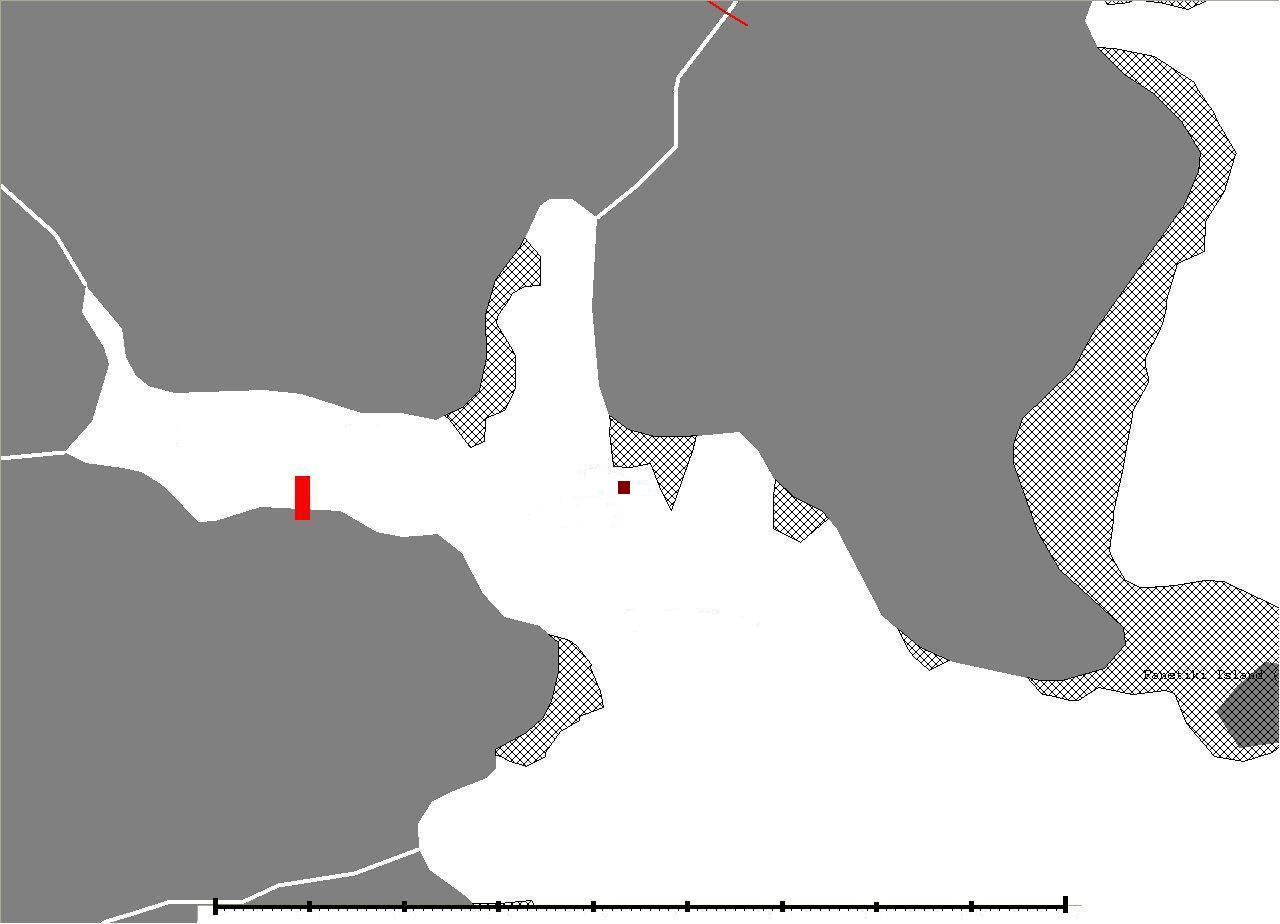
\includegraphics[width=0.5\linewidth]{images/sampling_site} 

}

\caption{Location of sampling site....}\label{fig:location}
\end{figure}
\hypertarget{cross-references}{%
\subsection{Cross-references}\label{cross-references}}

External images and R figures can be referenced with \texttt{\textbackslash{}@ref(fig:\textless{}label\textgreater{})}, where \texttt{\textless{}label\textgreater{}} is the name of the code chunk (in the above example its \emph{location}). These label names should \textbf{not contain underscores} to separate words, use hyphens here instead. Note that figures need to have a caption to be numbered and for cross-referencing, The caption is also set in the chunk option with \texttt{fig.cap=\textquotesingle{}Your\ caption\textquotesingle{}}.

Cross-references to individual sections can simply be made by placing the name of the section into squared brackets, e.g.~a link to the \protect\hyperlink{discussion}{Discussion} is made via \texttt{{[}Discussion{]}}.

Tables require also a label and table caption for cross-referencing as figures. But here, the cross-reference contains a \texttt{tab:} in \texttt{\textbackslash{}@ref(tab:\textless{}name\textgreater{})}) instead of a \texttt{fig:}. Also, captions of tables produced with R cannot be set in the chunk options as for figures but in the R functions directly (see examples in the \protect\hyperlink{results}{Results}).

This is for example a cross-reference to table \ref{tab:kable1} in the \protect\hyperlink{using-the-knitr-and-kableextra-packages}{Using the \texttt{knitr} and \texttt{kableExtra} packages} chapter.

\textbf{Important note}: Labels for tables produced with R Markdown syntax have to be set with \LaTeX notation, hence, the cross-reference has to be also in \LaTeX (see for an example \protect\hyperlink{r-markdown-table}{R Markdown table}).

\hypertarget{formulas}{%
\subsection{Formulas}\label{formulas}}

Use mathematics in R Markdown as usual using the dollar sign \texttt{\$}; either in \textbf{inline mode} with one dollar sign \(E = mc^2\) or in \textbf{display mode} with two \texttt{\$\$}: \[E = mc^2\]
Important to note: do not leave a space between the \texttt{\$} and your mathematical notation.

Alternatively, you can use \LaTeX for more control and when equations are more complicated. \LaTeX equations are also automatically numbered, which is useful if you have many equations and want to cross-reference them (note: if you set a star after the \texttt{\{equation*\}}, as in the last equation, the number is suppressed). The equation label needs to be written in \LaTeX with \texttt{\textbackslash{}label\{eq:label\}}, which follows the \texttt{\textbackslash{}begin\{equation\}} element (see eq. \eqref{eq:mean}):
\begin{equation} \label{eq:mean}
  \bar{X} = \frac{\sum_{i=1}^n X_i}{n} 
\end{equation}
Formulas and corresponding explanations should be integrated into the sentence and, thus, end with a comma or period. Here comes an example:

If the random variable \(Y\) follows a standard normal distribution, i.e. \(Y \sim N(0,1)\), it's density function can be described with
\begin{equation} \label{eq:density-norm}
  f_{Y}(y)=\varphi(y) \stackrel{\mathrm{def}}{=} \frac{1}{\sqrt{2 \pi}} \exp \left\{ -\frac{y^2}{2} \right\}, y \in \mathbb{R}.
\end{equation}
\(\pi\) represents the circle number or Ludolph's number. The function
\begin{equation*}
  F_{Y}(y) = \Phi(y) \stackrel{\mathrm{def}}{=} \int_{-\infty}^y \varphi(x) \,\mathrm{d}x, \quad y \in \mathbb{R},
\end{equation*}
represents then the distribution function of \eqref{eq:density-norm}.

\hypertarget{results}{%
\section{Results}\label{results}}

The result chapter is of great importance in an empirical study and should comprise a good mix of text, tables and figures. Use your research questions and hypothesis for structuring this chapter to provide the reader some structure and not loose the red thread.

Figures and tables should be continuously numbered and referred to in the main text. \LaTeX places figures and tables automatically were they fit best, which is sometimes on the next page. This is fine since they are cross-referenced anyway.

Tables have generally a caption at the top, while figures have a caption at the bottom. This has to be considered in some of the R functions (see below).

\hypertarget{tables}{%
\subsection{Tables}\label{tables}}

\hypertarget{r-markdown-table}{%
\subsubsection{R Markdown table}\label{r-markdown-table}}

Table \ref{tab:rmd_tab} is a R Markdown table including a caption and label for cross-referencing. The caption is set with \texttt{Table:\ ...} and can come before or after the table. You do not need so set a number as \LaTeX will care of the numbering as well as the placing. Also note that the caption requires no quotation marks.

The label is set \textbf{right after} the table caption with \texttt{\textbackslash{}label\{tab:name\}}. \textbf{Note here} that this is \LaTeX notation, where brackets are \textbf{curly}, not round! Also when cross-referencing R Markdown tables use the \LaTeX notation \texttt{\textbackslash{}ref\{tab:name\}} (i.e., no \texttt{@} and curly brackets).
\begin{longtable}[]{@{}lcr@{}}
\caption{This is a table written in R Markdown.\label{tab:rmd_tab}}\tabularnewline
\toprule
A & New & Table\tabularnewline
\midrule
\endfirsthead
\toprule
A & New & Table\tabularnewline
\midrule
\endhead
left-aligned & centre-aligned & right-aligned\tabularnewline
\$123 & \$456 & \$789\tabularnewline
\emph{italics} & normal & \textbf{boldface}\tabularnewline
\bottomrule
\end{longtable}
\hypertarget{tables-generated-with-r}{%
\subsubsection{Tables generated with R}\label{tables-generated-with-r}}

\hypertarget{using-the-knitr-and-kableextra-packages}{%
\paragraph{\texorpdfstring{Using the \texttt{knitr} and \texttt{kableExtra} packages}{Using the knitr and kableExtra packages}}\label{using-the-knitr-and-kableextra-packages}}

~

Table \ref{tab:kable1} is an example when using \texttt{knitr::kable} to generate the table and \texttt{kableExtra} to modify it. \texttt{knitr::kable()} has an explicit argument named \texttt{caption} where you can place your caption text.
\begin{table}

\caption{\label{tab:kable1}This is a table produced with knitr and modified with kableextra.}
\centering
\fontsize{9}{11}\selectfont
\begin{tabular}[t]{lrrrrrr}
\toprule
\multicolumn{1}{c}{\textbf{ }} & \multicolumn{4}{c}{\textbf{Group 5}} & \multicolumn{2}{c}{\textbf{Group 6}} \\
\cmidrule(l{3pt}r{3pt}){2-5} \cmidrule(l{3pt}r{3pt}){6-7}
\multicolumn{1}{c}{ } & \multicolumn{2}{c}{Group 1} & \multicolumn{2}{c}{Group 2} & \multicolumn{1}{c}{Group 3} & \multicolumn{1}{c}{Group 4} \\
\cmidrule(l{3pt}r{3pt}){2-3} \cmidrule(l{3pt}r{3pt}){4-5} \cmidrule(l{3pt}r{3pt}){6-6} \cmidrule(l{3pt}r{3pt}){7-7}
  & mpg & cyl & disp & hp & drat & wt\\
\midrule
Mazda RX4 & 21.0 & 6 & 160 & 110 & 3.90 & 2.620\\
Mazda RX4 Wag & 21.0 & 6 & 160 & 110 & 3.90 & 2.875\\
Datsun 710 & 22.8 & 4 & 108 & 93 & 3.85 & 2.320\\
Hornet 4 Drive & 21.4 & 6 & 258 & 110 & 3.08 & 3.215\\
Hornet Sportabout & 18.7 & 8 & 360 & 175 & 3.15 & 3.440\\
\bottomrule
\multicolumn{7}{l}{\textit{Note: }}\\
\multicolumn{7}{l}{Your comments go here.}\\
\end{tabular}
\end{table}
\hypertarget{the-xtable-package}{%
\paragraph{\texorpdfstring{The \texttt{xtable} package}{The xtable package}}\label{the-xtable-package}}

~

\href{https://cran.r-project.org/web/packages/xtable/vignettes/xtableGallery.pdf}{xtable} has become increasingly popular but is not as easy to use as \texttt{knitr::kable}. For instance, when using the default settings the table caption is placed \emph{below} the table (see Table \ref{tab:xtable1}). Also, the label for cross-referencing has to be set inside the \texttt{xtable::xtable} function instead of the code chunk. And if you don't write \texttt{results=\textquotesingle{}asis\textquotesingle{}} inside the chunk options, you get the \LaTeX code for the table instead of the actual table in your PDF output file!
\begin{table}[ht]
\centering
\begin{tabular}{rrr}
  \hline
 & speed & dist \\ 
  \hline
1 & 4.00 & 2.00 \\ 
  2 & 4.00 & 10.00 \\ 
  3 & 7.00 & 4.00 \\ 
  4 & 7.00 & 22.00 \\ 
  5 & 8.00 & 16.00 \\ 
  6 & 9.00 & 10.00 \\ 
   \hline
\end{tabular}
\caption{This is a table made with 'xtable'.} 
\label{tab:xtable1}
\end{table}
The advantage of the \texttt{xtable} package for the advanced R/\LaTeX user is that \LaTeX code can directly be incorporated (see Table \ref{tab:xtable2}), and also the \texttt{xtable::print.xtable} function allows various additional settings.
\begin{table}[ht]
\centering
\caption{This is a table made with 'xtable' and modified with LaTeX Code and the print.xtable function.} 
\label{tab:xtable2}
\begin{tabular}{rrrrrrr}
  \toprule
 & {\Large{\bfseries{ mpg}}} & {\Large{\bfseries{ cyl}}} & {\Large{\bfseries{ disp}}} & {\Large{\bfseries{ hp}}} & {\Large{\bfseries{ drat}}} & {\Large{\bfseries{ wt}}} \\ 
  \midrule
{\emph{ Mazda RX4}} & 21.00 & 6.00 & 160.00 & 110.00 & 3.90 & 2.62 \\ 
  {\emph{ Mazda RX4 Wag}} & 21.00 & 6.00 & 160.00 & 110.00 & 3.90 & 2.88 \\ 
  {\emph{ Datsun 710}} & 22.80 & 4.00 & 108.00 & 93.00 & 3.85 & 2.32 \\ 
   \bottomrule
\end{tabular}
\end{table}
\hypertarget{figures}{%
\subsection{Figures}\label{figures}}

Figures can directly be produced with R and displayed here. Similar to external images, figure captions and labels are placed inside the chunk options for cross-referencing (see Figure \ref{fig:base-fig}).
\begin{figure}

{\centering \includegraphics[width=1\linewidth]{figures/base-fig-1} 

}

\caption{Relationship between horsepower and fuel economy}\label{fig:base-fig}
\end{figure}
Purely for demonstration purposes, figure \ref{fig:ggplot-fig} shows the same relationship but with \texttt{ggplot2} (automatically loaded with tidyverse) and in a different figure size.
\begin{figure}

{\centering \includegraphics{figures/ggplot-fig-1} 

}

\caption{Relationship between horsepower and fuel economy - displayed with ggplot2.}\label{fig:ggplot-fig}
\end{figure}
\hypertarget{discussion}{%
\section{Discussion}\label{discussion}}

Providing strict guidelines and rules for a good discussion is difficult. But the following recommendations might be helpful:
\begin{itemize}
\tightlist
\item
  The discussion follows the opposite structure than the introduction and should move from the specific to the more general topics.
\item
  Summary/recapitulation: You should start the discussion with a short summary of your main results and whether they support your hypothesis/hypotheses or not. Avoid here any statistical language as in the result section. You should again sketch out your line of argumentation in this section.
\item
  Continue with the main messages of your empirical or theoretical study or your literature review: What are new insights from your results?
\item
  Discussion of individual findings: expose results concisely and evaluate them critically. Potential questions that could be addressed here:
  \begin{itemize}
  \tightlist
  \item
    Are the findings convincing?
  \item
    In empirical studies: which conclusions about the problem studied can be drawn? What are the implications of your findings? Which theories and previous studies support your results, which are contradicting?
  \item
    In literature reviews: how many of the publications included in your analyses were high-quality and most recent? How many were outdated or had methodological flaws? Is there consensus across studies? Or are there group of studies that found different results?
  \item
    Which questions remain still unanswered? Which come out as important due to your findings?
  \end{itemize}
\item
  Point out the limitations of your study (assist reader in judging validity of findings). Are there any results that contradict your hypothesis and how can they be explained? Discuss to which extent your results can be generalized.
\end{itemize}
\hypertarget{conclusion}{%
\subsection{Conclusion}\label{conclusion}}
\begin{itemize}
\tightlist
\item
  Which \emph{take home messages} do you like to give the reader? What is the relevance of your study for future research and potential applications? Suggest issues for future research.
\item
  One \emph{final sentence} the complete the thesis.
\end{itemize}
\newpage

\hypertarget{references}{%
\section*{References}\label{references}}
\addcontentsline{toc}{section}{References}

\noindent

\setlength{\parindent}{-0.5cm}
\setlength{\leftskip}{0.5cm}
\setlength{\parskip}{8pt}

\hypertarget{refs}{}
\leavevmode\hypertarget{ref-kamm2000}{}%
Kamm J (2000) \emph{Evaluation of the Sedov-von Neumann-Taylor blast wave solution}. Technical Report LA-UR-00-6055. Los Alamos National Laboratory.

\leavevmode\hypertarget{ref-May1976}{}%
May RM (1976) Simple mathematical models with very complicated dynamics. \emph{Nature} 261(5560). Journal Article: 459--467. DOI: \href{https://doi.org/10.1038/261459a0}{10.1038/261459a0}.

\leavevmode\hypertarget{ref-RN410}{}%
Post E and Forchhammer MC (2002) Synchronization of animal population dynamics by large-scale climate. \emph{Nature} 420(6912). Journal Article: 168--171. DOI: \href{https://doi.org/10.1038/nature01064}{10.1038/nature01064}.

\indent
\setlength{\parindent}{17pt}
\setlength{\leftskip}{0pt}
\setlength{\parskip}{0pt}

\newpage

\appendix

\hypertarget{appendix}{%
\section{Appendix}\label{appendix}}

All relevant information has to be included in the main text. Irrelevant information as to be completely left out. Content that is related to the topic but not essential can be included in the appendix. Such could be the derivation of equations, additional information on statistical or laboratory analyses, source code of computer programs or any other comprehensive (data) material.

The appendix has to be similar to figures and tables cross-referenced and should \textbf{not} stand by itself. All figures and tables in the appendix should also have captions.

\hypertarget{figures-1}{%
\subsection{Figures}\label{figures-1}}
\begin{figure}

{\centering \includegraphics[width=1\linewidth]{figures/density-plot-1} 

}

\caption{Fuel economy in cities, grouped by the number of cylinders}\label{fig:density-plot}
\end{figure}
\hypertarget{tables-1}{%
\subsection{Tables}\label{tables-1}}
\begin{table}[ht]
    \caption{Descriptive statistics of .... }
    \label{tab:apptable}
    \begin{center}
        {\footnotesize
        \begin{tabular}{l|cccccccccc}
        \hline \hline
                        & 3m    & 6m    & 1yr   & 2yr   & 3yr   & 5yr   & 7yr   & 10yr  & 12yr  & 15yr   \\
            \hline
                Mean   & 3.138 & 3.191 & 3.307 & 3.544 & 3.756 & 4.093 & 4.354 & 4.621 & 4.741 & 4.878  \\
                Median & 3.013 & 3.109 & 3.228 & 3.490 & 3.680 & 3.906 & 4.117 & 4.420 & 4.575 & 4.759  \\
                Min    & 1.984 & 1.950 & 1.956 & 2.010 & 2.240 & 2.615 & 2.850 & 3.120 & 3.250 & 3.395  \\
                Max    & 5.211 & 5.274 & 5.415 & 5.583 & 5.698 & 5.805 & 5.900 & 6.031 & 6.150 & 6.295  \\
                StD    & 0.915 & 0.919 & 0.935 & 0.910 & 0.876 & 0.825 & 0.803 & 0.776 & 0.768 & 0.762  \\
            \hline \hline
        \end{tabular}}
    \end{center}
\end{table}
\newpage

\hypertarget{acknowledgements}{%
\section{Acknowledgements}\label{acknowledgements}}

I want to thank the following people \ldots{}

\newpage

\hypertarget{declaration-of-authorship}{%
\section{Declaration of Authorship}\label{declaration-of-authorship}}

\emph{I hereby declare in lieu of an oath that I have authored the present \thesistype{} independently and
without use of others than the indicated sources - in particular of internet sources other than
the one mentioned in the list of sources. The \thesistype{} has not been submitted by me
to any other examination procedure before. The submitted written version corresponds to the
version on the electronic storage medium. I agree that the \thesistype{} may be published.}
\vspace{0.5cm}

{[}\emph{Hiermit erkläre ich an Eides statt, dass die vorliegende \thesistype{} von mir selbständig
verfasst wurde und ich keine anderen als die angegebenen Hilfsmittel -- insbesondere
keine im Quellenverzeichnis nicht benannten Internet--Quellen -- benutzt habe und die
Arbeit von mir vorher nicht einem anderen Prüfungsverfahren eingereicht wurde. Die
eingereichte schriftliche Fassung entspricht der auf dem elektronischen Speichermedium.
Ich bin damit einverstanden, dass die \thesistype{} veröffentlicht wird.}{]}
\vspace{1cm}

Hamburg, \thesisdate{}
\vspace{3cm}

. . . . . . . . . . . . . . . . . . . . . . . . . . . . . . .
\vspace{0.1cm}

\thesisauthor{}

% change rmd_files in `_bookdown.yml` files to determine order
% note that references and appendix are also contained here.



\end{document}
